% !TeX program = xelatex
\documentclass[11pt]{report}

\renewcommand{\thesection}{\arabic{section}}
\usepackage{multicol}
\usepackage{pgfplots}
\usepackage{amsmath}
\usepackage{siunitx}
\usepackage{graphicx}
\usepackage{wrapfig}
\usepackage{subcaption}
\usepackage[siunitx, RPvoltages]{circuitikz}
\usepackage[includefoot, bottom=0.5cm, right=1.5cm, left=1.5cm, top=1.5cm]{geometry}
\usepackage{enumitem}
\usepackage{lipsum}
\usepackage{fontspec}
\usepackage{sectsty}
\usepackage{float}
\usepackage{setspace}
\usepackage[]{indentfirst}
\usepackage[backend=biber, style=numeric]{biblatex}

\addbibresource{bjt.bib}
\graphicspath{{images}}
\pgfplotsset{width=10cm,compat=1.9, table/search path={data}}
\usetikzlibrary{intersections}
\usepgfplotslibrary{fillbetween}
\defaultfontfeatures{Ligatures=TeX}
\setmainfont{Arial}
\newfontfamily{\timesNewRoman}{Times New Roman}
\newenvironment{abstractText}{\timesNewRoman\itshape}{\par}
\onehalfspacing
\subsectionfont{\fontsize{12pt}{15}\rmfamily\selectfont}

\begin{document}
	\title{\textbf{EEE109 Lab Report:}\\ BJT and Amplifiers}
	\author{Felix Lianto (2362727)\\
		[1cm]{\small Instructors: Guanying Chu, Bing Han, Jiaqi Lu}}
	\maketitle

\sectionfont{\itshape\fontsize{14pt}{15}\timesNewRoman\selectfont}
\section{Abstract}
\begin{abstractText}
	Bipolar Junction Transistors, abbreviated as BJTs, are circuit elements that can functionally act as an amplifier or a switch. They are heavily used in all sorts of computer-related circuitry, such as digital logic circuits. This report explores these electronic components from its working principle to its applications, to which it found that the transistor works similarly to the diode, but thanks to its two junctions compared to one in the semiconductor diode, it has the ability to amplify signals as well. Furthermore, due to having 2 pn-junctions very close to each other, the transistor has 3 working regions that are frequently utilized in circuit design, namely being the cutoff and saturation region for the switch, and the forward-active region for the amplifier.
\end{abstractText}

\rmfamily
\sectionfont{\fontsize{14pt}{15}\rmfamily\selectfont}
\section{Introduction}
Transistor is a three terminal circuit element mainly used to control current flow within an electronic circuit \autocite{subramaniNanoelectronicApplicationsCarbon2023}. Aside from being a current flow controller, transistors also have other use cases such as switches, amplifiers, oscillators, and much more \autocite{subramaniNanoelectronicApplicationsCarbon2023}. Thus, transistors have become a fundamental component in modern technology due to its many functionalities, yet still hold so much potential for improvement in the future \autocite{caoPublisherCorrectionFuture2023}. Hence, this report aims to give an introduction to one such transistor known as the Bipolar Junction Transistor, abbreviated as BJT, as well as circuit applications in the form of a switch, a common emitter amplifier, and and an emitter-follower amplifier.

\subsection{Bipolar Junction Transistors}
Before introducing BJTs, a foundation in semiconductor diodes will be necessary to understand further discussion. To keep it simple and intuitive, semiconductor diodes are circuit elements that can block current from going one way. It does this by utilizing doped semiconductor materials placed very closely to each other, which creates a depletion region that can block current in one direction, and conduct in another. The relation between current and voltage conducted by the diode can be expressed using the Shockley diode equation
\begin{equation}
	i_D = I_s\left(e^{\frac{v_D}{nV_T}}-1\right)
\end{equation}
where
\begin{align*}
	i_D&: \text{Current flowing through the diode,} \\
	v_D&: \text{Voltage across the diode,} \\
	n&: \text{Ideality factor,} \\
	V_T&: \text{Thermal voltage ($\SI{25.3}{\milli\volt}$ for room temperature), and} \\
	I_S&: \text{Reverse-bias saturation current.}
\end{align*}
To keep our calculations simple, this report will be assuming an approximate, ideal diode. This means that the $-1$ contribution will not be taken into consideration, as well as setting $n=1$ for an ideal diode. Hence, the equation that will be utilized for this report is
\begin{equation}
	i_D = I_se^{\frac{v_D}{V_T}}
\end{equation}

Transistors can largely be divided into two categories, Field-Effect Transistors (FET), which controls current flow by the voltage at the gate node, and Bipolar Junction Transistors (BJT), the main discussion for this report, which controls by the current at the base terminal \autocite{subramaniNanoelectronicApplicationsCarbon2023}. The BJT consists of 3 doped semiconductor materials placed very close to each other, as shown in Figure \ref{npnandpnp}, resembling that of placing 2 semiconductor diodes side by side. These then forms the terminals for the BJT, namely the collector, the base, and the emitter \autocite{subramaniNanoelectronicApplicationsCarbon2023}, differentiated by the current arrow in the circuit element representation, as displayed in Figure \ref{circuitsymbols}.

\begin{figure}[h]
	\centering
	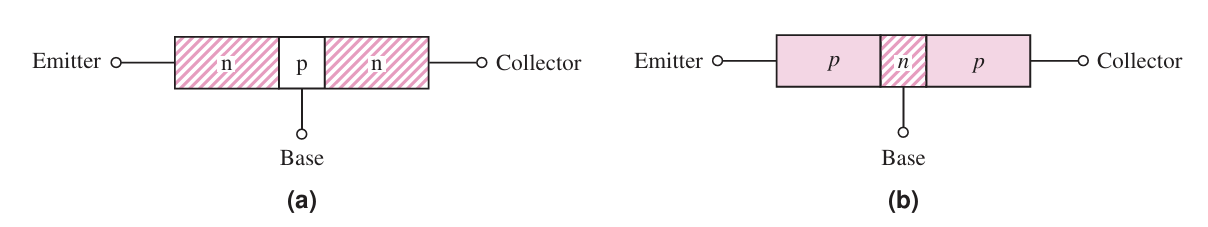
\includegraphics[scale=0.6]{npnandpnp.png}
	\caption{The npn (left) and pnp (right) transistor \autocite{neamenMicroelectronicsCircuitAnalysis2007}}
	\label{npnandpnp}
\end{figure}
\begin{figure}[h]
	\centering
	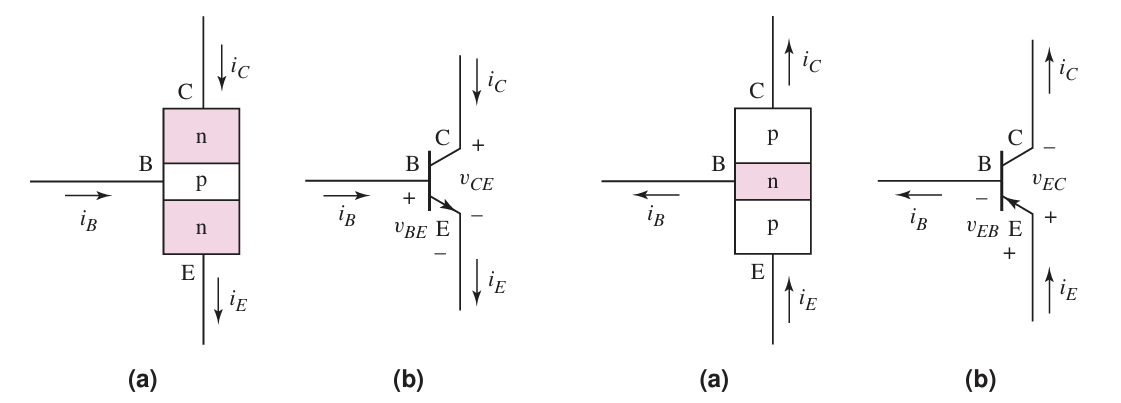
\includegraphics[scale=0.6]{circuitsymbols.png}
	\caption{BJT circuit symbols \autocite{neamenMicroelectronicsCircuitAnalysis2007}}
	\label{circuitsymbols}
\end{figure}

From these terminals, the BJT can be subdivided into the npn transistor and the pnp transistor \autocite{shurBipolarTransistors2003}. As the name suggests, the difference between these two transistors are its flipped doped-semiconducting material. The main difference between the two is that npn transistors' current flow from the collector to the emitter, while pnp transistors flow from the emitter to the collector \autocite{waseemUnderstandingNPNVs2023}, as illustrated in Figure \ref{circuitsymbols}. This is due to their differences in the majority charge carriers, as the majority charge carriers in an npn transistor are electrons, while a pnp transistor has holes.

This difference is significant when it comes to its applications. The npn transistor is mainly used for its near-instantaneous switching and high-frequency operation thanks to its majority charge carriers being electrons \autocite{waseemUnderstandingNPNVs2023}. This has led to its frequent applications as amplifiers, logic gates, and LEDs \autocite{waseemUnderstandingNPNVs2023}. While the npn transistor has its uses, the pnp transistor also has applications in circuit design, specifically as current sources, pull-up circuits, and high-side loads \autocite{waseemUnderstandingNPNVs2023}. Though, for this experiment, it will only consider the npn transistor, as it is the main transistor that was utilized.

It might be helpful to think of the BJT as 2 semiconductor diodes in opposite directions of each other, with the base terminal in the middle, as shown in Figure \ref{twoDiodes}. From this figure, it can be seen that, much like the diode, the BJT behaves differently depending on the current flowing through its terminals. These behaviors are often grouped as 'regions of operation', to which the BJT has 3; the cutoff, saturation, and active region.
\begin{figure}[h]
	\centering
	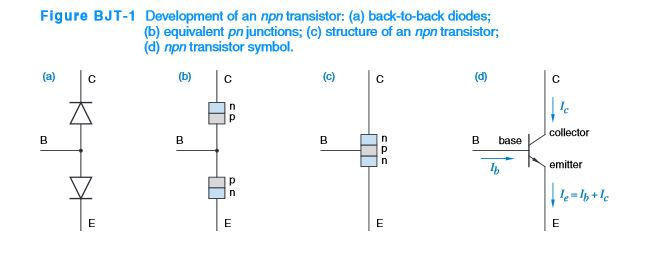
\includegraphics[scale=0.8]{2diodes.jpg}
	\caption{Two diodes representation \autocite{vasiliyAnswerWhyCant2013}}
	\label{twoDiodes}
\end{figure}

If both diodes are working in reverse bias, then no current will be conducted through either of them, as they will be treated as open circuits. This region is known as the cutoff region, and it happens when the base current is smaller than the collector and emitter current. If both diodes are in forward bias, then the transistor will conduct the maximum possible current, which is some multiple smaller than the base current. Analogously, the cutoff region can be thought of as the transistor being 'fully off', and the saturation region as 'fully on' \autocite{Lab2BJT}.

However, when it comes to the active region, this is where the back-to-back diode model fails, as it does not take into account the geometry of the BJT transistor \autocite{vasiliyAnswerWhyCant2013}. Namely, since the base's width is usually made to be small, the current will be inaccurately reflected by the diode model \autocite{vasiliyAnswerWhyCant2013}. To illustrate this forward-active region, graphing the collector-emitter and base-emitter curves will be useful, displayed in Figure X. From the figure, we can see that the collector current is close to a linear function after a certain value of $V_{CE}$. Hence, we can represent this mathematically \autocite{Lab2BJT} as
\begin{equation}
	I_C = \beta I_B
\end{equation}
where $\beta$ is some constant, commonly referred to as the common-emitter current gain.

\begin{figure}[h]
	\centering
	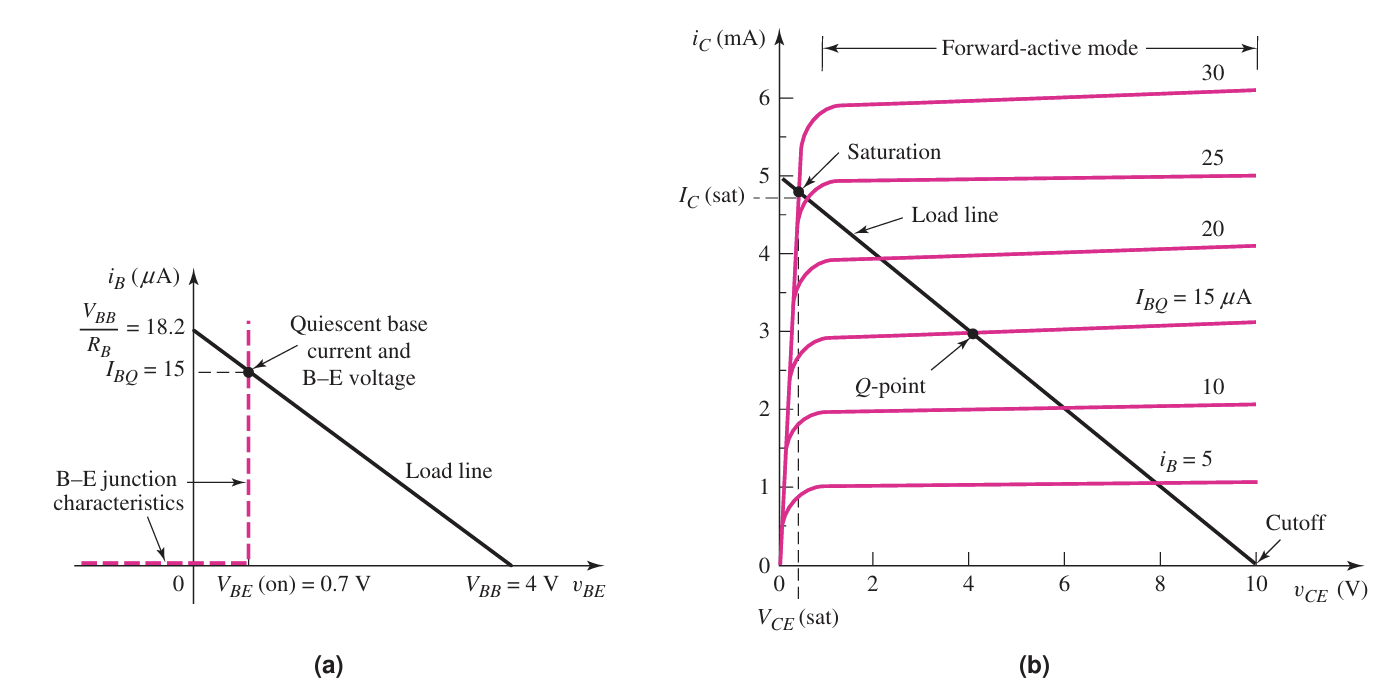
\includegraphics[scale=0.5]{loadLine.png}
	\caption{Graphical representation of the BE and BC junctions \autocite{neamenMicroelectronicsCircuitAnalysis2007}}
	\label{loadLine}
\end{figure}

This experiment will utilize the 2N3904 npn transistor to analyze its behavior under the IV analyzer, a potentiometer circuit, as well as running LTspice simulations on it too. It is hypothesized that the result will follow a fast growing curve until a certain point where it starts linearly increasing. This will closely mimic the regions of operation principle as explained previously.

\subsection{Common Applications of the BJT}
The BJT can be used in a variety of applications with regards to circuit design, as mentioned briefly in the previous section on npn and pnp transistors. However, two applications stand out to be the most common, which are switches and amplifiers.

For BJT switches, this can be accomplished through the cutoff and saturation operation region of the transistor. Specifically, by adjusting the base current, the BJT can be forced into either cutoff mode, where no current can flow, or saturation mode, where the current is allowed to be flowed through. A simple circuit of this can be seen in Figure \ref{switchBJT}.

\begin{figure}[h]
	\centering
	\begin{circuitikz}[american]
		\draw (4, 1) node[npn] (Q1) {$Q_1$};
		\draw (0, 0) to[vsource, l=$V_{CC}$] (0, 6)
			-- (2, 6) to [R, a=$R_1$] (2, 4) -- (2, 2)
			to [pR, a=$R_2$, n=pot] (2, 0) -- (0, 0);
		\draw (2, 6) to[short, f=$I_C$] (4, 6) 
			to[R, l=$R_C$, v=$V_{R_C}$] (4, 4)
			to[empty led, l=$LED_1$, v=$V_{LED_1}$] (4, 2) -- (Q1.collector);
		\draw (pot.wiper) -- (Q1.base);
		\draw (Q1.collector) ++(1, -0.1) to[open, v^=$V_{CE}$] ++(0, -1.65);
		\draw (Q1.emitter) -- (4, 0) -- (2, 0);
		
		\draw (Q1.collector) to[short, -o] ++(1, 0);
		\draw (4, 0) to[short, -o] ++(1, 0);
	\end{circuitikz}
	\caption{BJT as a Switch}
	\label{switchBJT}
\end{figure}

From this figure, it is expected that the LED will light up when the switch is closed. Precisely, assuming the circuit elements are ideal, when the transistor is cutoff, $V_{CE} = 0$ and the LED will be off. While when the transistor is saturated, $V_{CE} = V_{RC} = \SI{15}{\volt}$ and $I_C = \SI{15}{\milli\ampere}$ and the LED will be on. Further details will be provided in the following sections.

To amplify a current signal, recall the forward-active region of the BJT. It has been established that the collector current is some multiple of the base current, dictated by the common-emitter current gain. This property allows the collector current to be amplified by a constant gain, hence the function of amplifying a current signal. Several methods exist that can actualize this property, however for this report, we will only look at two amplifier circuits, being the transistor amplifier and the emitter follower amplifier.

When it comes to circuitry, both amplifiers are very similar, as shown in Figure \ref{bjtAmplifiers}. However, the differing element in both circuits is the output voltage. In the transistor amplifier, the voltage level at the collector terminal is the output voltage, while the output voltage in the emitter follower amplifier is at the emitter terminal itself.

\begin{figure}[h]
	\centering
	\begin{subfigure}{0.5\textwidth}
		\centering
		\begin{circuitikz}[american, scale=0.9, transform shape]
			\draw (6, 3) node[npn] (npn1) {};
			\draw (0, -1) to[vsource, l=$V_{CC}$] (0, 6)
				-- (4, 6) to[R, l=$R_1$] (4, 4)
				-- (4, 3) to[short, f=$I_B$] (npn1.base);
			\draw (4, 3) to[C, a=$C_1$] (2, 3)
				to[sV<=$V_{in}$] (2, -1) -- (0, -1);
			\draw (4, 3) to[R, l=$R_2$] (4, -1) -- (2, -1);
			
			\draw (4, 6) to[short, f=$I_C$] (6, 6)
				to[R, a=$R_L$] (npn1.collector);
			\draw (npn1.collector) to[short, -o] ++(2, 0) node[above]{$V_{out}$}
				to[open, v=$V_{CE}$] ++(0, -3);
				
			\draw (npn1.emitter) to[short, f=$I_E$] (6, 1)
				to[R, a=$R_E$] (6, -1) -- (4, -1);
			\draw (6, 1) to[short, -o] (8, 1)
				to[C, a=$C_2$] (8, -1) -- (6, -1);
		\end{circuitikz}
		\caption{Transistor amplifier}
		\label{transistorAmplifier}
	\end{subfigure}%
	\begin{subfigure}{0.5\textwidth}
		\centering
		\begin{circuitikz}[american, scale=0.9, transform shape]
			\draw (6, 3) node[npn] (npn1) {};
			\draw (0, -1) to[vsource, a=$V_{CC}$] (0, 6)
			-- (4, 6) to[R, l=$R_1$] (4, 4)
			-- (4, 3) to[short, f=$I_B$] (npn1.base);
			\draw (4, 3) to[C, a=$C_1$] (2, 3)
			to[sV<=$V_{in}$] (2, -1) -- (0, -1);
			\draw (4, 3) to[R, l=$R_2$] (4, -1) -- (2, -1);
			
			\draw (4, 6) to[short, f=$I_C$] (6, 6)
			-- (npn1.collector);
			
			\draw (npn1.emitter) to[short, f=$I_E$] (6, 1)
			to[R, a=$R_E$] (6, -1) -- (4, -1);
			\draw (6, 1) to[C, a=$C_2$, -o] (8, 1) node[above]{$V_{out}$}
				to[R, l=$R_L$] (8, -1) -- (6, -1);
		\end{circuitikz}
		\caption{Emitter follower amplifier}
		\label{emitterFollowerAmplifier}
	\end{subfigure}
	\caption{Common BJT amplifier circuits}
	\label{bjtAmplifiers}
\end{figure}

This report will report on various features of these amplifier circuits, as well as measuring their voltage gains from various instruments.

\section{Research Aims}
\underline{This experiment aims to fulfill the following objectives:}
\begin{enumerate}
	\itemsep 0em
	\item Investigate the working principle behind the BJT,
	\item Explore the influence of the base and collector terminal to the emitter terminal,
	\item Illustrate how DC analysis is performed on a BJT switching circuit,
	\item Investigate voltage gains from various instruments within a transistor amplifier circuit, and
	\item Investigate the current gain in an emitter-follower circuit when the emitter resistance is varied.
\end{enumerate}

\section{Experimental Procedures}
The laboratory activities were executed under the NI Elvis III platform, with the following components:

This experiment was done in 4 parts, where a certain area pertaining to the BJT was explored in each part.
\subsection{Bipolar Junction Transistors}
This activity was completed with these electrical components:
\begin{itemize}
	\itemsep 0em
	\item 2N3904 npn Bipolar Junction Transistor
	\item $\SI{33}{\kilo\ohm}$ Resistor
	\item $\SI{100}{\ohm}$ Resistor
	\item $\SI{1}{\kilo\ohm}$ Potentiometer (provided by the platform's proto-board)
\end{itemize}

This section aims to analyze the resulting differences when the base current and collector voltage was varied. To accomplish this, two methods were utilized, the manual method and the automatic method. The automatic method involved the current-voltage analyzer instrument built into the NI Elvis III system, while the manual method consisted of measuring in a real circuit, shown in Figure \ref{procedures1-2}. The plot for both methods are then exported and displayed in the next section.
\begin{figure}[h]
	\centering
	\begin{circuitikz}[american]
		\draw (3, 4) node[npn] (npn1) {$Q_1$};
		\draw (0, 0) to[vsource, l=$V_B$] (0, 4)
			to[R, l=$\SI{33}{\kilo\ohm}$, f_=$I_B$] (2, 4) -- (npn1.base);
		\draw (npn1.collector) to[short, f<=$I_C$] ++(2, 0)
			to[pR, name=pot] node[above right, yshift=1cm, xshift=0.2cm] {$\SI{1}{\kilo\ohm}$} ++(0, -2)
			to[short, -o] ++(0, -0.5);
		\draw (pot.wiper) -- ++(1, 0)
			to[R, l=$\SI{100}{\ohm}$] ++(0, -2)
			to[vsource, l=$\SI{15}{\volt}$, invert] ++(0, -1.5) |- (0, 0);
		\draw (npn1.emitter) |- (0, 0);
		\draw (npn1.collector) to[open] ++(1, 0)
			to[open, v=$V_{CE}$] ++(0, -1.5);
		\draw (npn1.emitter) to[short, -o] ++(1, 0);
	\end{circuitikz}
	\caption{Circuit for instrumentation measurement}
	\label{procedures1-2}
\end{figure}

\subsection{BJT as a Switch}
This section will not involve any real-world experiments, it will instead only focus on analysis of the BJT circuit shown in Figure \ref{switchBJT}. This subsection will demonstrate how to determine the collector-emitter voltage in cutoff and saturation region, as well as the saturated voltage across the collector resistor $R_C$ and the saturated collector current $I_C$. The list of numerical values for each component will be listed below, while a step-by-step analysis of the circuit will be given in the next section.
\begin{align*}
	V_{CC} &= \SI{15}{\volt} \\
	R_1 &= \SI{10}{\kilo\ohm} \\
	R_2 &= \SI{1}{\kilo\ohm} \\
	R_C &= \SI{1}{\kilo\ohm} \\
	V_{LED_1} &= \SI{1.8}{\volt} \text{ (Forward voltage of the LED)}
\end{align*}

\subsection{Transistor Amplifiers}
This activity was done with the following electrical components:
\begin{itemize}
	\itemsep 0em
	\item 2N3940 npn Bipolar Junction Transistor
	\item $\SI{560}{\ohm}$ Resistor
	\item $\SI{1}{\kilo\ohm}$ Resistor
	\item $\SI{8.2}{\kilo\ohm}$ Resistor
	\item $\SI{18}{\kilo\ohm}$ Resistor
	\item $\SI{1}{\micro\farad}$ Capacitor
	\item $\SI{100}{\micro\farad}$ Capacitor
\end{itemize}

The circuit was constructed similarly to Figure \ref{transistorAmplifier} on the NI Elvis III breadboard. Figure \ref{numericalTransistorAmplifier} shows the same circuit, but with its numerical values instead of symbolic values.
\begin{figure}[h]
	\centering
	\begin{circuitikz}[american, scale=0.9, transform shape]
		\draw (6, 3) node[npn] (npn1) {};
		\draw (0, -1) to[vsource, l=$\SI{15}{\volt}$] (0, 6)
		-- (4, 6) to[R, a=$\SI{18}{\kilo\ohm}$] (4, 4)
		-- (4, 3) to[short, f=$I_B$] (npn1.base);
		\draw (4, 3) to[C, a=$\SI{1}{\micro\farad}$] (2, 3)
		to[sV<=$V_{in}$] (2, -1) -- (0, -1);
		\draw (4, 3) to[R, l=$\SI{8.2}{\kilo\ohm}$] (4, -1) -- (2, -1);
		
		\draw (4, 6) to[short, f=$I_C$] (6, 6)
		to[R, l=$\SI{1}{\kilo\ohm}$] (npn1.collector);
		\draw (npn1.collector) to[C, a=$\SI{1}{\micro\farad}$, -o] ++(2, 0) node[above]{$V_{out}$}
		to[open, v=$V_{CE}$] ++(0, -3);
		
		\draw (npn1.emitter) to[short, f=$I_E$] (6, 1)
		to[R, a=$\SI{560}{\ohm}$] (6, -1) -- (4, -1);
		\draw (6, 1) to[short, -o] (8, 1)
		to[C, l=$\SI{100}{\micro\farad}$] (8, -1) -- (6, -1);
	\end{circuitikz}
	\caption{Transistor amplifier}
	\label{numericalTransistorAmplifier}
\end{figure}
For the AC source, the Function Generator was utilized to provide the values, while the DC voltage source was provided by the proto-board on the NI Elvis III.
Then, to measure the waveforms, 2 channels of the oscilloscope was wired to the AC source and the $V_{out}$ node. Both of these results are then displayed in the following section. Moreover, this circuit will also be analyzed by a bode analyzer, with similar procedures as the oscilloscope. The results of the bode analyzer will be compared against the oscilloscope, to draw conclusions based on it, as per the research aim outlined earlier.

Furthermore, a replica of this experiment was also done in LTspice, so there would be values to compare to between the real circuit and a simulated, ideal one. The following section will also comment on the difference between these two.

\subsection{Emitter Follower Amplifier}
This part of the experiment will only involve simulating the emitter follower amplifier circuit in LTspice. The circuit will be really similar to the transistor amplifier circuit, however we are only measuring the emitter terminal's voltage with respect to the ground rather than the collector terminal.

Similar to the transistor amplifier, we will analyze this circuit in terms of its gain, however we will measure the current gain instead of the voltage gain now. The numerical circuit simulated for this section is provided in Figure \ref{numericEmitterFollowerCircuit}, where the input voltage has an amplitude of $\SI{2.5}{\volt}$ and a frequency of $\SI{10}{\kilo\hertz}$.
\begin{figure}[h]
	\centering
	\begin{circuitikz}[american, scale=0.9, transform shape]
		\draw (6, 3) node[npn] (npn1) {};
		\draw (0, -1) to[vsource, a=$\SI{12}{\volt}$] (0, 6)
		-- (4, 6) to[R, l=$R_1$] (4, 4)
		-- (4, 3) to[short, f=$I_B$] (npn1.base);
		\draw (4, 3) to[C, a=$C_1$] (2, 3)
		to[sV<=$V_{in}$] (2, -1) -- (0, -1);
		\draw (4, 3) to[R, l=$R_2$] (4, -1) -- (2, -1);
		
		\draw (4, 6) to[short, f=$I_C$] (6, 6)
		-- (npn1.collector);
		
		\draw (npn1.emitter) to[short, f=$I_E$] (6, 1)
		to[R, a=$R_E$] (6, -1) -- (4, -1);
		\draw (6, 1) to[C, a=$C_2$, -o] (8, 1) node[above]{$V_{out}$}
		to[R, l=$R_L$] (8, -1) -- (6, -1);
	\end{circuitikz}
	\caption{Emitter follower amplifier}
	\label{numericEmitterFollowerCircuit}
\end{figure}
The current gain will be calculated by dividing the current flowing through the load resistor on the bottom right by the current flowing into the base terminal of the BJT. We will observe this gain as the resistor on the emitter terminal $R_E$ is varied, to which its result will be plotted on a graph in the upcoming section.

\section{Results and Discussion}
The experimental results will be divided into 4 sections, following the lab script structure.
\subsection{Bipolar Junction Transistors}
The experiment aims to uncover the behavior of the bipolar junction transistor through DC sweep analysis. Figure \ref{sect1-1} shows the result of the sweep analyses through the automatic method, which is by the IV analyzer. As expected, it follows the curve in Figure \ref{loadLine}, as per the hypothesis. However, something peculiar about the experimental result is that it is overall slightly larger than the simulated results. In fact, the LTspice simulation here shows a nearly straight line in its active region, compared to the more majorly sloped real BJTs. One plausible reason for this discrepancy is the Early voltage.
\begin{figure}[h]
	\centering
	\begin{tikzpicture}[scale=0.9]
		\begin{axis}[
			xlabel={Collector-emitter Voltage [V]},
			ylabel={Collector Current [A]},
			ymax=0.02,
			ymajorgrids,
			no markers,
			grid style={dashed},
			legend to name=ideal,
			legend columns=5,
			legend entries={$\SI{15}{\micro\ampere}$, $\SI{26}{\micro\ampere}$, $\SI{37}{\micro\ampere}$, $\SI{48}{\micro\ampere}$, $\SI{59}{\micro\ampere}$},
			cycle list={
				{blue, mark=*},
				{red, mark=square},
				{black, mark=+},
				{green, mark=o},
				{cyan, mark=|}
			}
			]
			
			\addplot +[name path=real1] table [x=v1, y=Ic1]{iv2.dat};
			\addplot +[name path=real2] table [x=v2, y=Ic2]{iv2.dat};
			\addplot +[name path=real3] table [x=v3, y=Ic3]{iv2.dat};
			\addplot +[name path=real4] table [x=v4, y=Ic4]{iv2.dat};
			\addplot +[name path=real5] table [x=v5, y=Ic5]{iv2.dat};
			
			\addplot +[name path=ideal1, densely dashed] table [x=v1, y=Ic1]{iv1.dat};
			\addplot +[name path=ideal2, densely dashed] table [x=v1, y=Ic2]{iv1.dat};
			\addplot +[name path=ideal3, densely dashed] table [x=v1, y=Ic3]{iv1.dat};
			\addplot +[name path=ideal4, densely dashed] table [x=v1, y=Ic4]{iv1.dat};
			\addplot +[name path=ideal5, densely dashed] table [x=v1, y=Ic5]{iv1.dat};
			
			\addplot [fill=blue!50, fill opacity=0.3] fill between[of=ideal1 and real1];
			\addplot [fill=red!50, fill opacity=0.3] fill between[of=ideal2 and real2];
			\addplot [fill=black!50, fill opacity=0.3] fill between[of=ideal3 and real3];
			\addplot [fill=green!50, fill opacity=0.3] fill between[of=ideal4 and real4];
			\addplot [fill=cyan!50, fill opacity=0.3] fill between[of=ideal5 and real5];
		\end{axis}
		\node[anchor=north] at (current axis.below south){\ref{ideal}};
	\end{tikzpicture}
	\caption{DC Sweep Analysis of the BJT through the IV analyzer (Dashed: LTspice Simulation, Solid: Real Experimentation)}
	\label{sect1-1}
\end{figure}

The Early effect is the phenomenon where the collector current increases as the base-collector voltage increases \autocite{EarlyEffect2024,54NonidealEffects}. This phenomenon occurs due to the depletion region within the base-collector junction increasing, leading to a decrease in the charge carrier section of the base terminal \autocite{EarlyEffect2024}. This decrease leads to a smaller chance of recombination within the smaller base region, as well as an increase in charge gradient across the base, both of which leads to an increase in the collector current \autocite{EarlyEffect2024}. The Early effect is something that running simulations would fail to catch, as it is something that happens exclusively with a non-ideal diode \autocite{54NonidealEffects}. However, note that there are several other factors that could have influenced this result too, such as temperature and the common-emitter gain.

Recall that the collector current is equal to the Shockley diode equation, which means the thermal voltage $V_T$ will come to affect the resulting voltage, among other factors. More generally, when working with real circuit elements, they are subjected to manufacturing limitations. These limitations are often what causes instability in values that, at least in circuit analysis on paper, would be constant. These changes are not reflected in the simulation, as it proves too great a challenge to model perfectly.

This experiment also considered the manual method of multimeter measurement as well. Figure \ref{sect1-2} shows those results from measurement. Similar to the automatic method, it was found that the experimental results are also overall higher than the simulation. However, due to some problems working with the potentiometer, the graph was missing some entries. For future attempts on this experiment, it is recommended that two variable voltage sources should be used instead, as the potentiometer have its limits and can be a bit unreliable.
\begin{figure}[h]
	\centering
	\begin{tikzpicture}
		\begin{axis}[
				xlabel={Collector-emitter Voltage [V]},
				ylabel={Collector Current (A)},
				ymajorgrids,
				legend to name=myplot,
				legend entries={
					$\SI{2.38}{\volt}$, $\SI{4.08}{\volt}$, $\SI{5.76}{\volt}$
				}
				grid style={dashed},
				unbounded coords=jump,
				cycle list={
					{blue,mark=*},
					{red,mark=square},
					{brown!60!black,mark=otimes*,
						mark options={fill=brown!40},
					}
				}
			]
			
			\addplot +[name path=real1] table [x=Vce,y=Ic1] {realIV1-2.dat};
			\addplot +[name path=real2] table [x=Vce,y=Ic2] {realIV1-2.dat};
			\addplot +[name path=real3] table [x=Vce,y=Ic3] {realIV1-2.dat};
			
			\addplot +[name path=ideal1, densely dashed] table [x=Vce,y=Ic1] {idealIV1-2.dat};
			\addplot +[name path=ideal2, densely dashed] table [x=Vce,y=Ic2] {idealIV1-2.dat};
			\addplot +[name path=ideal3, densely dashed] table [x=Vce,y=Ic3] {idealIV1-2.dat};
			
			\addplot [fill=blue!50, fill opacity=0.3] fill between[of=ideal1 and real1];
			\addplot [fill=red!50, fill opacity=0.3] fill between[of=ideal2 and real2];
			\addplot [fill=brown!50, fill opacity=0.3] fill between[of=ideal3 and real3];
		\end{axis}
		\node[anchor=north] at (current axis.below south){\ref{myplot}};
	\end{tikzpicture}
	\caption{DC Sweep Analysis of the BJT through the Multimeter (Dashed: LTspice Simulation, Solid: Real Experimentation)}
	\label{sect1-2}
\end{figure}

\subsection{BJT as a Switch}
This section will provide a sufficient analysis of the circuit in Figure \ref{switchBJT}, under the assumptions stated previously. To calculate the collector-emitter voltage in cutoff mode, notice that no current will run through the BJT, in other words, $I_C = 0$. This means that the $R_C$ resistor must not have any current flowing through it, meaning that there is no voltage drop across it. Thus, the cutoff common-emitter voltage must be equal to $V_{CC}$, which means $V_{CE} = \SI{15}{\volt}$. Naturally, this also means that the LED is in reverse bias, meaning that in this state, it is not lit.

To calculate in the saturation region, an assumption will be made, which is the value of the saturated collector-emitter voltage. According to the lab manual for this experiment and taking the median from a datasheet for a common npn transistor \autocite{onsemiGeneralPurposeLow,Lab2BJT}, the value of $\SI{0.1}{\volt}$ will be the assumption made. Then, to calculate the voltage across the collector resistor, we can take the difference between $V_{CC}$ and $V_{LED_1} + V_{CE}$, which outputs the voltage drop of $\SI{13.1}{\volt}$. For the collector current, we can utilize Ohm's law to calculate the resulting value of $\SI{13.1}{\milli\ampere}$. This also confirms the state of the LED being ON, since the current is positive.

These results also match with the simulations, with only an error of $2.63\%$. This error margin could be due to any number of factors, such as a weak assumption about the saturated collector-emitter voltage, among many others. Regardless, this subsection has achieved in showing how DC analysis is done with a BJT circuit such as this one.

\subsection{Transistor Amplifiers}
This section will present its findings from the experiment listed previously. Figure \ref{sect3-1} compares the input and output waveforms from both the experiment and simulation. As expected of an amplifier, the output waveform is significantly larger than the input waveform. Additionally, while the real and simulated waves are not in phase, most likely due to an poorly chosen trigger condition not letting the waveform to properly align itself \autocite{strattonAnswerOscilloscopeRun2018}, the amplitude of the waveforms are not radically different between the real and the simulated one. The tiny difference between these two would most likely be caused by internal resistance from other circuit elements.
\begin{figure}[h]
	\centering
	\begin{tikzpicture}
		\begin{axis}[
			xlabel={Voltage [V]},
			ylabel={Time [ms]},
			ymajorgrids,
			no markers,
			grid style={dashed},
			legend to name=oscilloscope,
			legend columns=5,
			legend entries={Real voltage, Simulated voltage},
			cycle list={
				{blue, mark=*},
				{red, mark=square}
			},
			x post scale=2
			]
			
			\addplot +[name path=real1, each nth point={100}] table [x=t1, y=v1]{realOscilloscope.dat};
			\addplot +[name path=ideal1, densely dashed] table [x=t, y=v1]{idealOscilloscope.dat};
			
			\addplot +[name path=real2, each nth point={100}] table [x=t2, y=v2]{realOscilloscope.dat};
			\addplot +[name path=ideal2, densely dashed] table [x=t, y=v2]{idealOscilloscope.dat};
			
			\addplot [fill=blue!50, fill opacity=0.3] fill between[of=real1 and real2];
			\addplot [fill=red!50, fill opacity=0.3] fill between[of=ideal1 and ideal2];
		\end{axis}
		\node[anchor=north] at (current axis.below south){\ref{oscilloscope}};
	\end{tikzpicture}
	\caption{Resulting waveforms from the oscilloscope (Bigger: output, Smaller: input)}
	\label{sect3-1}
\end{figure}

One interesting observation to be made here is that both the input and output waveforms are out of phase with each other. This is due to the relationship between the base terminal voltage and the collector-emitter voltage. When the base voltage increases, $I_C$ will increase, leading to a smaller $V_C = V_{out}$ as $V_{CC}$ is constant, and vice versa \autocite{storrCommonEmitterAmplifier2013}. Thus, the inverting amplifier behavior occurs and the output waveform is $180$ degrees out of phase.

We now consider the gains of the circuit calculated from the oscilloscope and the bode analyzer. The gain calculated from the oscilloscope, referred to as the linear gain, is calculated using the formula \autocite{Lab2BJT};
\begin{equation}
	\text{Linear Gain in } dB = 20\log_{10}\frac{V_{out}}{V_{in}}
\end{equation}
For the experimental waveform, the linear gain measured from the peak-to-peak voltage value is $\SI{29.2}{\decibel}$, while the simulation was measured at $\SI{32.3}{\decibel}$, which means a rough error percentage of $9.60\%$. Meanwhile, the bode gain measured from the analyzer returned a value of $\SI{17.28}{\decibel}$ in the experiment and $\SI{32.79}{\decibel}$ in the simulation, an astounding error of $48.2\%$. This result is way out of the expectation, as both of the gains should be equal in theory. Even more confusingly, there seems to be a huge disparity in magnitude between the real and simulated results, as shown in Figure \ref{sect3-2}. One plausible explanation to the limited magnitude shown is due to parasitic effects of the junctions in the transistor. These effects can reduce the expected gain significantly and is often not accounted for in simulations, thus giving rise to the disparity observed in Figure \ref{sect3-2}.
\begin{figure}[h]
	\centering
	\begin{tikzpicture}
		\begin{axis}[
			xlabel={Frequency [Hz]},
			ylabel={Magnitude [dB]},
			no markers,
			ymajorgrids,
			grid style={dashed},
			legend to name=bode,
			legend columns=5,
			legend entries={Real, Ideal},
			cycle list={
				{blue, mark=*}
			},
			xmode=log,
			y filter/.code={\pgfmathparse{20*log10(\pgfmathresult)}}
			]
			
			\addplot +[name path=realMag] table [x=Freq, y=Mag]{realBode.dat};
			\addplot +[name path=idealMag, densely dashed] table [x=Freq, y=Mag]{idealBode.dat};
			
			\addplot [fill=blue!50, fill opacity=0.3] fill between[of=realMag and idealMag];
		\end{axis}
		\node[anchor=north] at (current axis.below south){\ref{bode}};
	\end{tikzpicture}
	\caption{Magnitude result from the experiment and simulation bode analysis}
	\label{sect3-2}
\end{figure}

\subsection{Emitter Follower Amplifier}
This section will present its current gain findings after simulating the emitter follower circuit on LTspice. Figure \ref{sect4} shows the growth of the current gain with respect to the resistance $R_E$.
\begin{figure}[h]
	\centering
	\begin{tikzpicture}
		\begin{axis}[
			xlabel={Emitter Terminal Resistance [\si{\kilo\ohm}]},
			ylabel={Magnitude [dB]},
			no markers,
			ymajorgrids,
			grid style={dashed},
			y filter/.code={\pgfmathparse{20*log10(\pgfmathresult)}}
			]
			
			\addplot table [x=RE, y=Gain]{emitterFollower.dat};
		\end{axis}
	\end{tikzpicture}
	\caption{Growth of the current gain against the emitter resistance}
	\label{sect4}
\end{figure}
Based on the figure, we can see that it follows the same logarithmic pattern as the voltage gain from the transistor amplifier circuit, as expected. This indicates that the load current is several times larger than the input current, which is what this circuit intends to do.

\section{Conclusion}
This report has outlined its findings with regards to the Bipolar Junction Transistor. Specifically, it has uncovered the working mechanisms behind the BJT, as well as some applications of them in circuits such as the amplifier circuits and the switch circuit. While the experiment is largely successful, there are some elements left to be desired. The discussion on the emitter-follower amplifier was rather brief, considering that it was not carried out experimentally. For future experiments, it would be preferable to build and test the emitter-follower circuit with a breadboard to have an interesting comparison between the two versions. This report hopes to have enlightened the reader in their electronic circuits study and further motivates them to experiment more with this modern technology.

\printbibliography

\end{document}